% Author:: Sebastien Badia (<seb@sebian.fr>)
% Date:: 2014-04-02 01:36:20 +0200
% vi: set ft=tex :

\documentclass[11pt,final,usepdftitle=false,handout]{beamer}
\mode<presentation>
\usetheme{lucasw}
\usepackage{tikz}
\usepackage{tikz-bpmn}
\usepackage{textpos}
\usepackage{verbatim}
\usetikzlibrary{positioning}
\hypersetup{pdftitle={OpenStack 101}}
\title[OpenStack 101]{OpenStack 101}
\author[Sébastien Badia]{Sébastien Badia\\ \texttt{sebastien.badia@enovance.com}\\[0.5em]}
\institute{eNovance -- 2 avril 2014\\
\vskip 3em
\begin{columns}[b]
\begin{column}{1cm}
\end{column}
\begin{column}{3cm}
	\centerline{
\includegraphics[height=1cm]{img/logo-eNovance-2011}}
\end{column}
\begin{column}{1cm}
\end{column}
\end{columns}
}
\date{}

\begin{document}
\frame{\titlepage}
\begin{frame}{Outline}
  \tableofcontents[hideallsubsections]
\end{frame}

% Author:: Sebastien Badia (<seb@sebian.fr>)
% Date:: 2014-04-02 01:36:20 +0200
% vi: set ft=tex :

\section{Cloud computing}
\begin{frame}{Outline}
    \tableofcontents[currentsection,hideallsubsections]
\end{frame}
\subsection{Definition}

\begin{frame}{Cloud computing}
\begin{block}{Definition}
Cloud computing is a model for enabling convenient, on-demand network access to a shared pool of configurable computing resources.
\end{block}
\begin{itemize}
  \item \textbf{On Demand}: Resources are dynamically created.
  \item \textbf{Multi-tenant}: Resources are shared between users.
  \item \textbf{Broad network access}: Network, standard mechanisms
  \item \textbf{Elasticity}: Infrastructure is flexible (grow/reduce).
  \item \textbf{Measured service}: Users pay what they use.
\end{itemize}
\end{frame}

\subsection{Cloud layers}
\begin{frame}{Cloud computing}
  \begin{textblock}{}(11,2)
      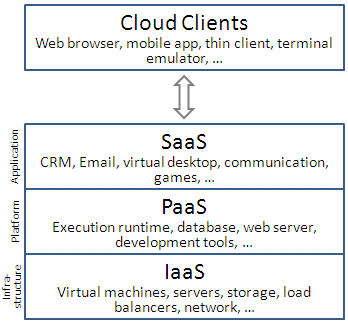
\includegraphics[width=8em]{img/Cloud_computing_layers}
  \end{textblock}
  \begin{itemize}
    \item Service models by the NIST\footnote{National Institute of Standards and Technology} (24 July 2011)
      \begin{itemize}
        \item Infrastructure as a service (IaaS)
        \medskip
        \item Platform as a service (PaaS)
        \medskip
        \item Software as a service (SaaS)
        \medskip
      \end{itemize}
    \item XaaS, a comprehensive taxonomy model
      \begin{itemize}
        \item Database as a service (DaaS)
        \medskip
        \item Network as a service (NaaS)
        \medskip
        \item …
      \end{itemize}
  \end{itemize}
\end{frame}

% Author:: Sebastien Badia (<seb@sebian.fr>)
% Date:: 2014-04-02 01:36:20 +0200
% vi: set ft=tex :

\section{Openstack}
\begin{frame}{Outline}
    \tableofcontents[currentsection,hideallsubsections]
\end{frame}
\subsection{Introduction}

\begin{frame}{OpenStack}
  \begin{textblock}{}(11,5)
      
\includegraphics[width=8em]{img/openstack-logo512}
  \end{textblock}
  \begin{itemize}
    \item Infrastructure as a service (\textbf{IaaS}) cloud middleware
      \medskip
    \item Open Source software (\textsl{\textbf{Apache} License})
      \medskip
    \item Derived from \textbf{Nebula} (\textsl{NASA}) and \textbf{Cloud Files} (\textsl{Rackspace})
      \medskip
    \item Written in \textbf{Python}
      \medskip
    \item Stable release: \textsl{\textbf{Havana} (October 13, 2014)}
      \medskip
  \end{itemize}
\end{frame}

\subsection{The foundation}
\begin{frame}{OpenStack Foundation}
  \begin{itemize}
    \item More than \textbf{9500 individual members}
      \medskip
    \item \textbf{100 countries}
      \medskip
    \item \textbf{850 different organizations}
      \medskip
    \item Secured more than \textbf{\$10 million} in funding
      \medskip
    \item Managed by 3 committee
  \end{itemize}
\end{frame}

\subsection{Committee}
\begin{frame}{Technical Committee}
  \begin{textblock}{}(11.5,-1)
      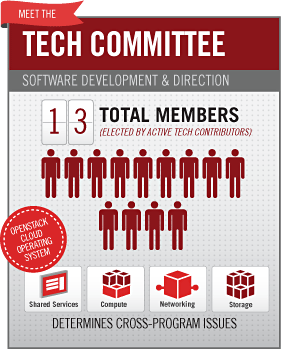
\includegraphics[width=7em]{img/osgraphictech}
  \end{textblock}
  \begin{itemize}
    \item TC manage software development and direction
      \medskip
    \item 13 members elected by active contributors
      \medskip
    \item Each OpenStack project has a PTL\footnote{Project Technical Leader}
      \medskip
    \item 5 are directly elected, and 8 are PTL
      \medskip
    \item Enforce OpenStack ideals (Openness, Transparency, Commonality, Integration, Quality)
  \end{itemize}
\end{frame}

\begin{frame}{Board of Directors}
  \begin{textblock}{}(11,6)
      
\includegraphics[width=7em]{img/osgraphicboard}
  \end{textblock}
  \begin{itemize}
    \item Protect, promote and empower OpenStack
      \medskip
    \item 24 members to provides strategic and financial oversight of Foundation
      \begin{itemize}
        \item 8 platinum (appointed by members)
        \item 8 gold (elected by member class) (eNovance \Smiley)
        \item 8 individual (elected by individual members)
      \end{itemize}
      \medskip
    \item Leaded by Alan Clark (Suse)
  \end{itemize}
\end{frame}

\begin{frame}{User Committee}
  \begin{textblock}{}(11,3.5)
      
\includegraphics[width=7em]{img/osgraphicusercommittee}
  \end{textblock}
  \begin{itemize}
    \item User advocacy and feedback, anybody can join
      \medskip
    \item Represent a broad set of enterprise, academic and service provider users
      \medskip
    \item Leaded by Tim Bell (CERN)
  \end{itemize}
\end{frame}

\begin{frame}{Community}
  \begin{textblock}{}(8,2)
      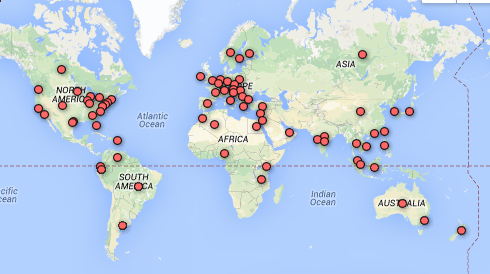
\includegraphics[width=12em]{img/oscommunity}
  \end{textblock}
  \begin{itemize}
    \item \textbf{Core} developers (elected) Grant for merging into master
      \medskip
    \item Anyone can contribute
      \begin{itemize}
        \item Code
        \item Documentation
        \item Support (irc, mail)
        \item …
      \end{itemize}
      \medskip
    \item \url{https://www.openstack.org/community/}
  \end{itemize}
\end{frame}

\begin{frame}{Releases cycle}
  \begin{center}
    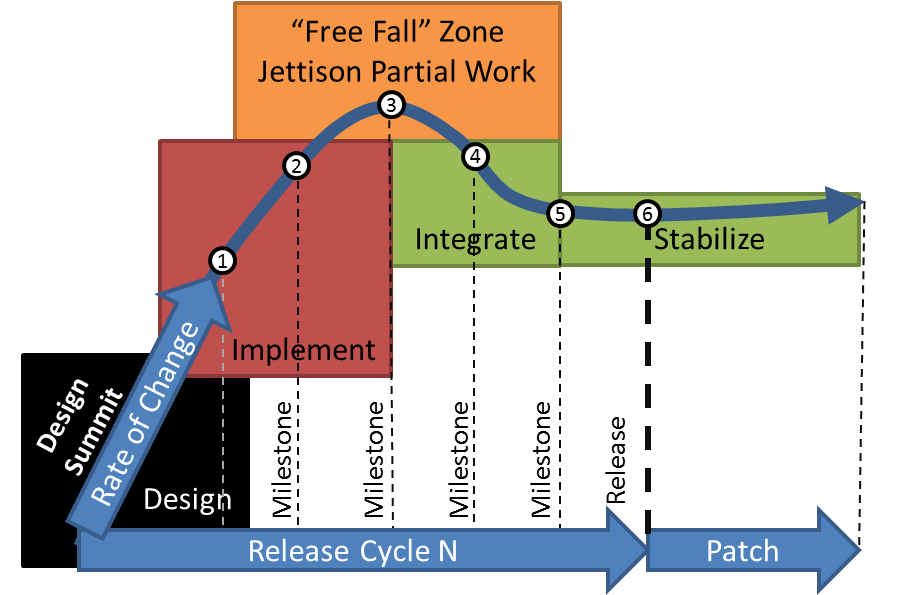
\includegraphics[width=20em]{img/os-releases}
  \end{center}
  \begin{itemize}
    \item A release every 6 months
    \item Alphabetical order \Smiley
    \item \url{https://wiki.openstack.org/Releases}
  \end{itemize}
\end{frame}

% Author:: Sebastien Badia (<seb@sebian.fr>)
% Date:: 2014-04-02 01:36:20 +0200
% vi: set ft=tex :

\section{Technical overview}
\begin{frame}{Outline}
    \tableofcontents[currentsection,hideallsubsections]
\end{frame}

\subsection{OpenStack IaaS}
\begin{frame}{OpenStack IaaS}
  \begin{itemize}
    \item Compute: Nova
    \item Images: Glance
    \item Identity: Keystone
    \item Storage: Swift (object), Cinder (block)
    \item Networking: Neutron
    \item Dashboard: Horizon
    \item Telemetry: Ceilometer
    \item Orchestration: Heat
  \end{itemize}
\end{frame}

\subsection{Openstack architecture}
\begin{frame}{OpenStack conceptual architecture}
  \begin{center}
    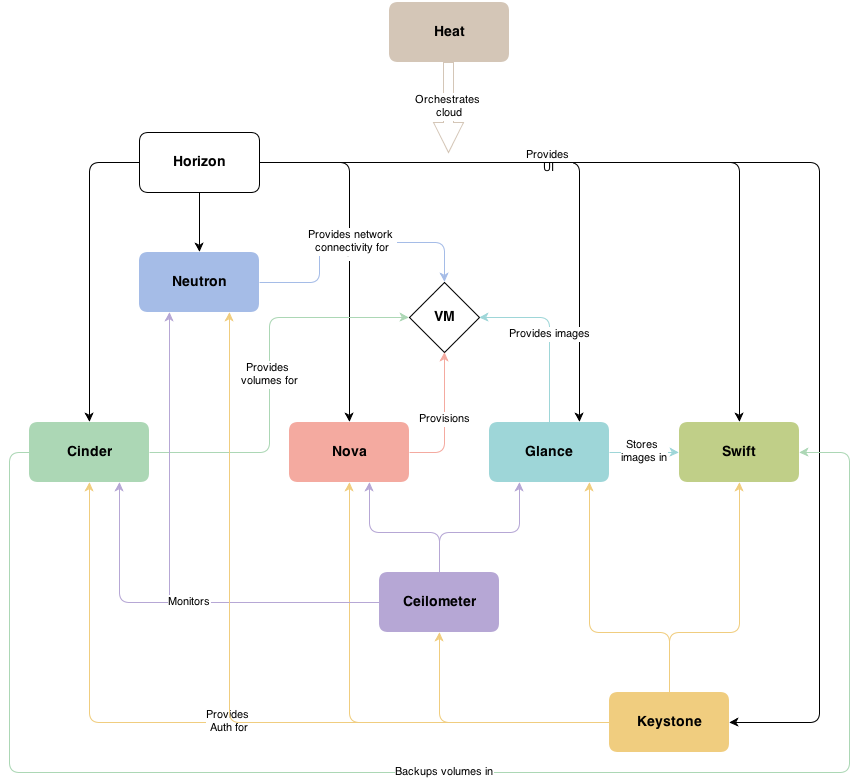
\includegraphics[width=22em]{img/openstack_havana_conceptual_arch}
  \end{center}
\end{frame}

\begin{frame}{OpenStack logical infrastructure}
  \begin{center}
    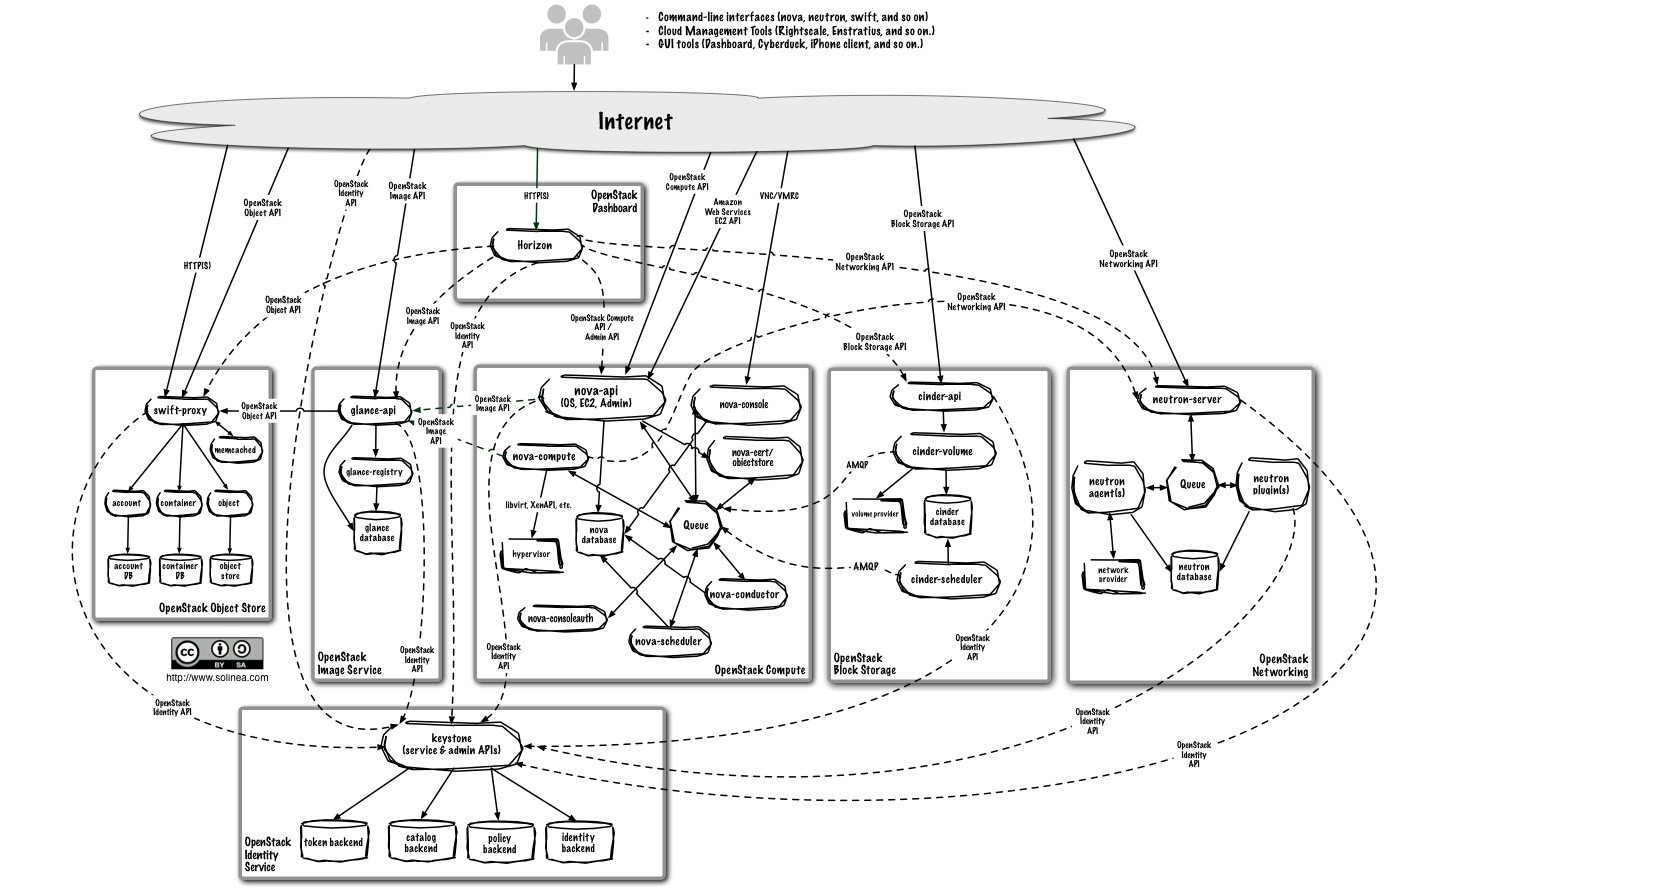
\includegraphics[width=38em]{img/openstack-arch-havana-logical-v1}
  \end{center}
\end{frame}

\subsection{Openstack Compute}
\begin{frame}{OpenStack Compute (\textsl{Nova})}
  \begin{textblock}{}(11,-2)
    
\includegraphics[width=7em]{img/compute}
  \end{textblock}
  \begin{itemize}
    \item Provision and manage virtual machines
      \medskip
    \item Hypervisor support: \textbf{XEN}/XCP, \textbf{KVM}, QEMU, LXC, ESX, ESXi\footnote{\url{http://wiki.openstack.org/HypervisorSupportMatrix}}
      \medskip
    \item OpenStack API (Compute API, Rackspace Cloud Server API)
      \medskip
    \item Support \textbf{live migration} (need a shared storage for instances) (\textsl{Ceph}, \textsl{Swift}, \textsl{NFS\footnote{\tiny{\url{http://docs.openstack.org/trunk/openstack-compute/admin/content/configuring-live-migrations.html}}}, GlusterFS\footnote{\tiny{\url{http://gluster.org/community/documentation/index.php/OSConnect}}}})
      \medskip
    \item Bare-metal, Cells
  \end{itemize}
\end{frame}
\begin{frame}{Nova Scheduler}
  \begin{textblock}{}(12,-2)
    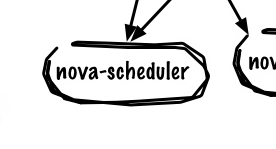
\includegraphics[width=7em]{img/nova-scheduler}
  \end{textblock}
  Nova-scheduler implements a few basic scheduling algorithms
  \begin{itemize}
    \item \textbf{Simple}: hosts whose \textbf{load is least} are chosen to run the instance. The load information may be fetched from a load balancer
    \item \textbf{Chance}: a compute host is chosen \textbf{randomly} across \textbf{availability zones}
    \item \textbf{Zone}: Similar to chance, but the compute host is chosen \textbf{randomly} from within a \textbf{specified zone}
  \end{itemize}
  \center
  \footnotesize
  \begin{tikzpicture}[node distance=1.2em]
  \tikzstyle{every task} = [thick,fill=white]
  \tikzstyle{every sequence} = [thick]
  \tikzstyle{every gateway} = [thick,fill=white]
  \tikzstyle{every event} = [thick,fill=white]
  \tikzstyle{end event} = [event,line width=2.5pt,fill=white]
    \node[event] (start) {};
    \node[task,right=of start] (rpc) {Rpc};
      \draw[sequence,->] (start) -- (rpc);
    \node[task,right=of rpc] (manager) {Scheduler manager};
      \draw[sequence,->] (rpc) -- (manager);
    \node[task,right=of manager] (multi) {Multi Scheduler};
      \draw[sequence,->] (manager) -- (multi);
    \node[task,right=of multi] (filter) {Filter Scheduler};
      \draw[sequence,->] (multi) -- (filter);
    \node[end event,right=of filter] (end) {};
      \draw[sequence,->] (filter) -- (end);
  \end{tikzpicture}
  \begin{itemize}
    \item Compute scheduler support \textttc{filtering} and \textttc{wheighting} to make informed decisions \footnote{\url{http://ibm.co/LUvm2n}}
    \item nova.scheduler.filters (core,compute,ram,cidr,different/same host) \footnote{\url{http://nova.openstack.org/devref/filter\_scheduler.html}}
  \end{itemize}
% shortURL: https://www.ibm.com/developerworks/mydeveloperworks/blogs/e93514d3-c4f0-4aa0-8844-497f370090f5/entry/openstack_nova_scheduler_and_its_algorithm27
\end{frame}

\begin{frame}{OpenStack Object storage (\textsl{Swift})}
  \begin{textblock}{}(11,7.8)
    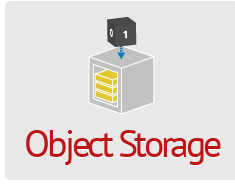
\includegraphics[width=6.5em]{img/swift}
  \end{textblock}
  \begin{itemize}
    \item Object storage (Swift): Redundant (Object/DB)\footnote{\url{http://swift.openstack.org/overview\_replication.html}} and scalable
      \medskip
    \begin{itemize}
      \item Storage via an API (\textbf{not a FS})
        \medskip
      \item \textbf{Long-term} storage system for \textbf{large amounts} of data
        \medskip
      \item Storage abstraction (Ring concept \footnote{\url{http://swift.openstack.org/overview\_ring.html}}, zone and weight of storage)
        \medskip
      \item Works with auth \textbf{token and HTTP API (RESTFull)}
        \medskip
      \item \textbf{Similarity with Amazon S3 (bucket)}
    \end{itemize}
  \end{itemize}
\end{frame}

\begin{frame}{OpenStack Image service (\textsl{Glance})}
  \begin{textblock}{}(11,8)
    
\includegraphics[width=7em]{img/image}
  \end{textblock}
  \begin{itemize}
    \item Image service (Glance): \textbf{Catalog} and \textbf{manage library}\\
      of \textbf{server images}
      \medskip
    \begin{itemize}
      \item Interaction between Nova-compute and Swift or Ceph
        \medskip
        \item Image format
        \begin{itemize}
          \item Conainer (bare,\textbf{ovf},aki,ari,ami)
          \item Disk (raw,vhd,vmdk,vdi,iso,\textbf{qcow2},aki,ari,\textbf{ami})\footnote{http://glance.openstack.org/formats.html}
        \end{itemize}
        \medskip
      \item Manageable by a CLI or an API Rest
        \medskip
      \item \textbf{Image Store} (\textbf{Ceph}, \textbf{Swift}, FS, S3)
        \medskip
      \item Glance support image caching \footnote{http://glance.openstack.org/cache.html}
    \end{itemize}
  \end{itemize}
\end{frame}

\begin{frame}{OpenStack Block storage (\textsl{Cinder})}
  \begin{textblock}{}(11,6)
    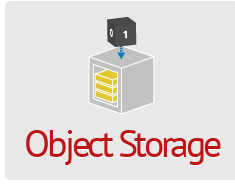
\includegraphics[width=6.5em]{img/swift}
  \end{textblock}
  \begin{itemize}
    \item Enables management of volumes, volume snapshots, and volume types
        \medskip
    \item Support: \textbf{RBD}, \textbf{iSCSI}, Sheepdog, AoE, LeftHand
        \medskip
    \item Similar to Amazon EBS
  \end{itemize}
\end{frame}

\begin{frame}{OpenStack Identity managment (\textsl{Keystone})}
  \begin{textblock}{}(0.3,3)
    
\includegraphics[width=2em]{img/identity-service}
  \end{textblock}
  \begin{itemize}
    \item Provide an \textbf{unified authentication} across \textbf{all openstack projects}
      \medskip
    \item Keystone concepts (\textsl{User managment})
      \medskip
      \begin{itemize}
        \item \textbf{Users}: a human user (login,password,email)
          \medskip
        \item \textbf{Tenants}: a group of users (project or organization)
          \medskip
        \item \textbf{Roles}: determine what operations an user is permitted to perform in a given tenant
          \medskip
      \end{itemize}
    \item Keystone manage also services (services,endpoint,catalog)
      \medskip
    \item OpenStack’s \textbf{Identity API} (XML/JSON API)
      \medskip
    \item Can be backed by LDAP
  \end{itemize}
\end{frame}

\begin{frame}{OpenStack Network (\textsl{Neutron})}
  \begin{itemize}
    \item Provides networking connectivity to VMs
      \medskip
    \item Manage L2 and L3 with a Rest API
      \medskip
    \item Networking backend by plugins:
      \medskip
      \begin{itemize}
        \item Open-vSwitch
      \medskip
        \item Linux Bridge
      \medskip
        \item OpenFlow
      \medskip
        \item Floodlight
      \medskip
        \item …
      \end{itemize}
  \end{itemize}
\end{frame}

\begin{frame}{OpenStack Telemetry (\textsl{Ceilometer})}
  \begin{itemize}
    \item Provide efficient collection of metering data, (CPU and network costs)
      \medskip
    \item Custom data by plug-ins.
      \medskip
    \item Produces signed metering messages that cannot be repudiated
  \end{itemize}
\end{frame}

\begin{frame}{OpenStack Orchestration (\textsl{Heat})}
  \begin{itemize}
    \item Provide a template-based for describing a cloud application.
      \medskip
    \item Integrated with all OpenStack ressources
      \medskip
    \item Provide advanced features (ha, auto-scaling, …)
      \medskip
    \item REST API,compatible with AWS CloudFormation
  \end{itemize}
\end{frame}

\begin{frame}{OpenStack Dashboard (\textsl{Horizon})}
  \begin{textblock}{}(12,12.3)
    
\includegraphics[width=1.7em]{img/dashboard}
  \end{textblock}
  \begin{table}[t]
    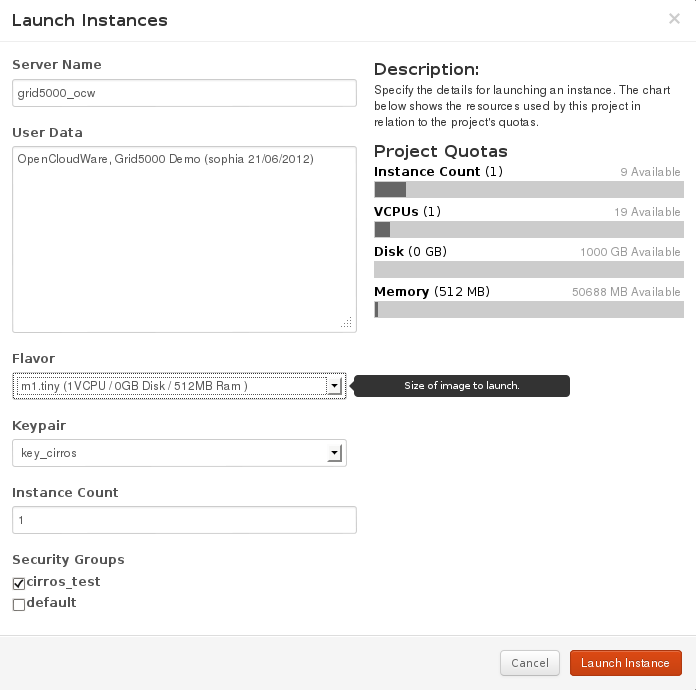
\includegraphics[width=16em]{img/dashboard_ocw}
  \end{table}
    \begin{itemize}
      \item Access and provision \textbf{cloud resources through a web portal}
      \item \textbf{Credentials}, \textbf{users} and \textbf{projects} management
      \item \textbf{Django module} for \textbf{easy} integration/creation
    \end{itemize}
\end{frame}

% Author:: Sebastien Badia (<seb@sebian.fr>)
% Date:: 2014-04-02 01:36:20 +0200
% vi: set ft=tex :

\section{Deploy, learn and tips}
\begin{frame}{Outline}
    \tableofcontents[currentsection,hideallsubsections]
\end{frame}

\begin{frame}{Development}
  \begin{textblock}{}(8,6)
    
\includegraphics[height=1.8cm]{img/logo-git.png}
  \end{textblock}
  \begin{textblock}{}(11.5,-3)
    
\includegraphics[height=2.5cm]{img/cat_review.jpg}
  \end{textblock}
  \begin{itemize}
    \item Integrated with launchpad (bug, milestone, cas)
    \item Code-review \url{https://review.openstack.org/}
      \begin{itemize}
        \item Git-review\footnote{\url{http://www.mediawiki.org/wiki/Gerrit/git-review}} (patch set lists / project setup / ease submit)
        \item In console, fgerrit\footnote{\url{https://github.com/pandemicsyn/fgerrit}}
      \end{itemize}
    \item Status \url{http://status.openstack.org/zuul/}
    \item Docs \url{http://wiki.openstack.org}
    \item IRC (oftc and freenode)
  \end{itemize}
\end{frame}

\begin{frame}{Git vs. Gerrit}
\vspace{-0.2cm}
\begin{center}
  \textbf{Git workflow}
\end{center}
\vspace{0.2cm}
\begin{center}
  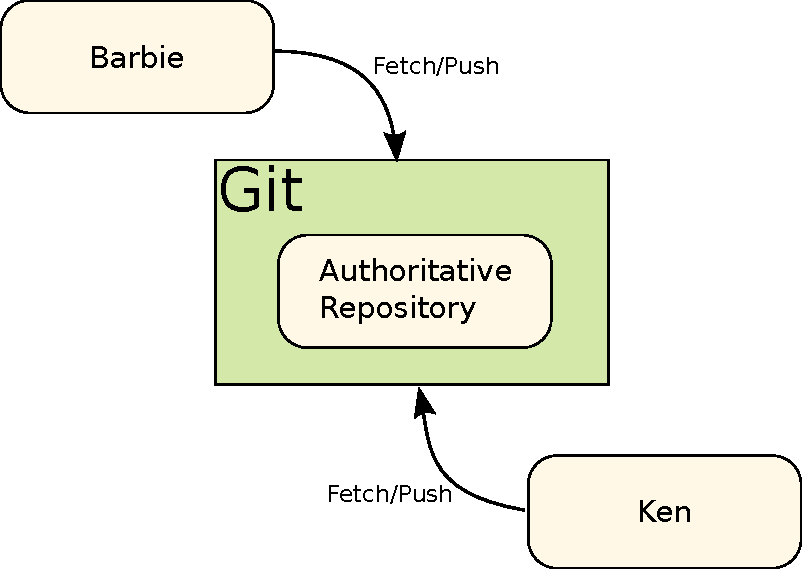
\includegraphics[height=6cm]{img/gerrit-workflow-classic.pdf}
\end{center}
\end{frame}

\begin{frame}{Git vs. Gerrit}
  \begin{center}
\textbf{Gerrit workflow}
\end{center}
\begin{center}
  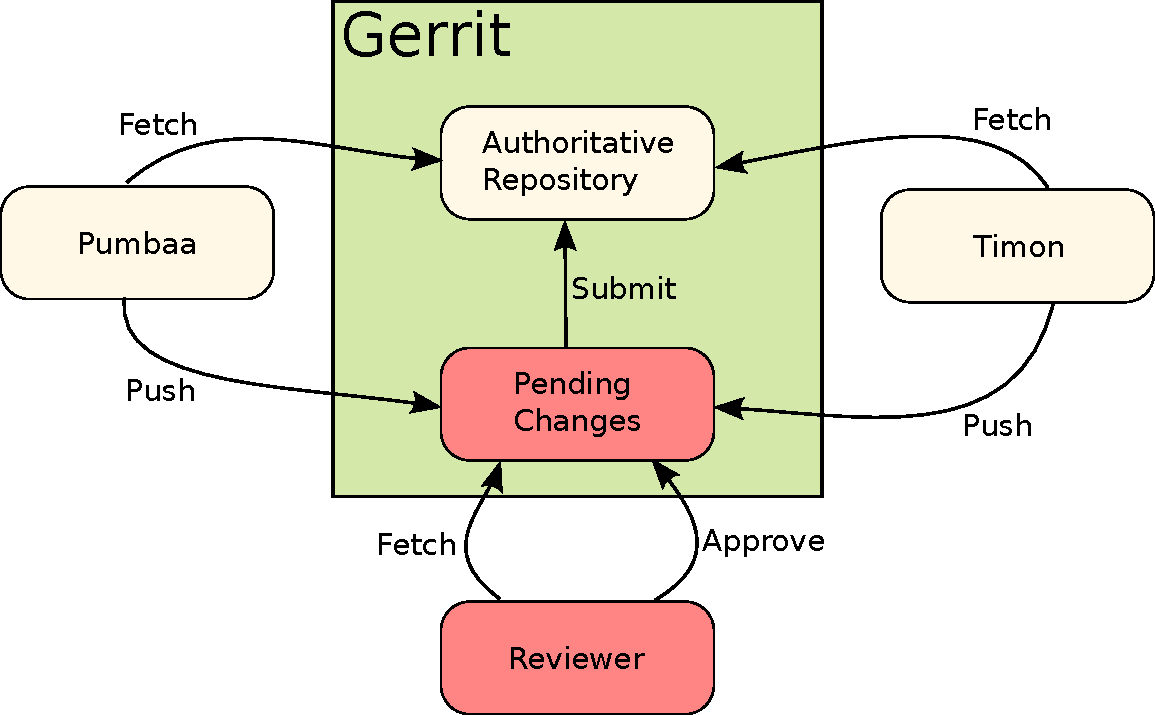
\includegraphics[height=7cm]{img/gerrit-workflow-gerrit.pdf}
\end{center}
\end{frame}

\begin{frame}{Gerrit and CI workflow}
  \begin{center}
    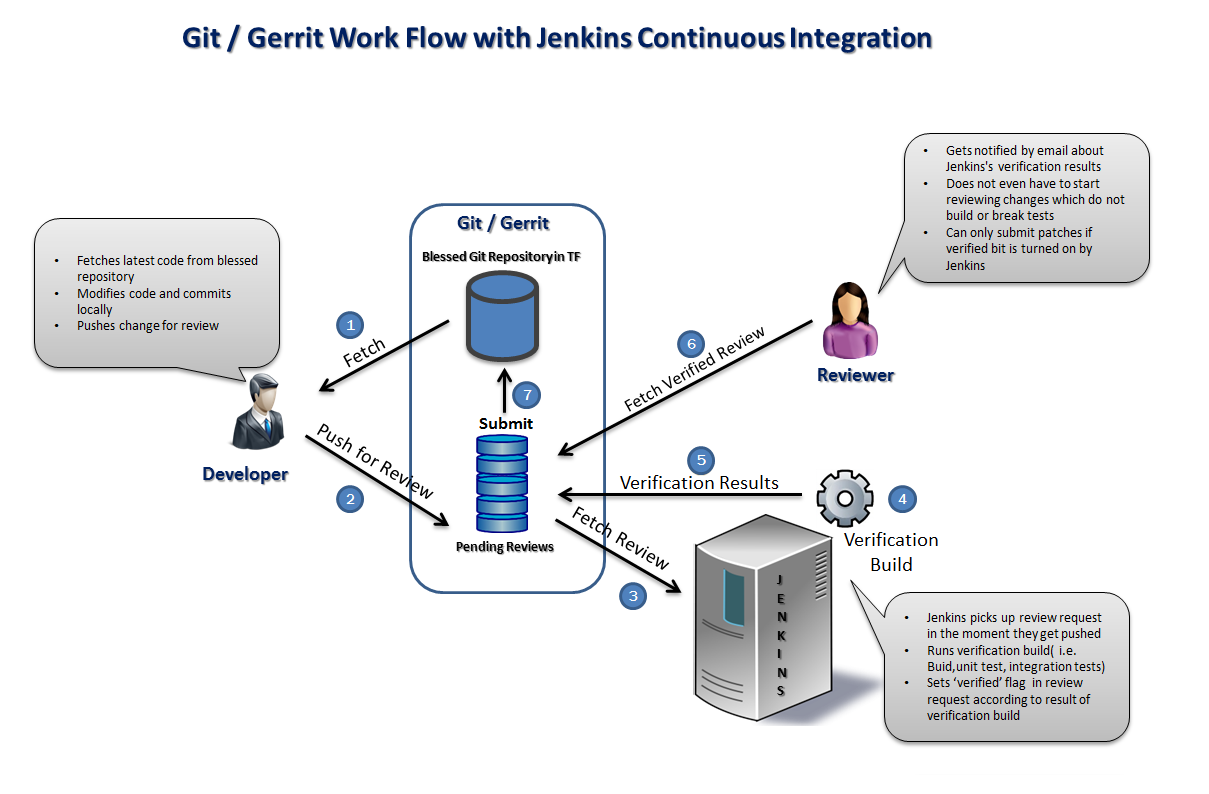
\includegraphics[height=7cm]{img/Git_gerrit_jenkins.png}
    \\ \tiny Courtesy of \url{http://blogs.collab.net/teamforge/teamforge-git-gerrit-integration-with-jenkins-ci}
  \end{center}
\end{frame}

\begin{frame}{Let's start}
  \begin{center}
    
\includegraphics[height=2cm]{img/silvio-berlusconi.jpg}
  \end{center}
  \begin{itemize}
    \item \url{https://github.com/openstack}
    \item \url{https://github.com/stackforge}
    \item \url{http://devstack.org/}
  \end{itemize}
\end{frame}

\subsection{Sources}
\begin{frame}{Sources, code}
\begin{itemize}
  \item OpenStack Wiki\\\url{http://docs.openstack.org/trunk/}\\\url{http://nova.openstack.org/devref/}
  \item Images\\\url{http://ken.pepple.info/}\\\url{http://openstack.org/}
  \item Slides \url{https://github.com/sbadia/slides}
\end{itemize}
\end{frame}


\end{document}
